
\documentclass{beamer}
\usepackage[latin1]{inputenc}
%\usetheme{Montpellier}
%\usetheme{Boadilla}
%\usecolortheme[RGB={204,51,255}]{structure}
%\usecolortheme[named=purple]{structure}
\usecolortheme[RGB={62,128,62}]{structure}
%\definecolor{dark}{rgb}{0.3,0.15,0.3}
%\definecolor{light}{rgb}{0.8,0.6,0.8}
%\definecolor{reddish}{rgb}{.5,0.15,0.15}
\definecolor{dark}{rgb}{0.5,0.3,0.4}
%\definecolor{light}{rgb}{0.8,0.6,0.8}
\definecolor{reddish}{rgb}{.7,0.25,0.25}
\definecolor{greenish}{rgb}{.25,0.7,0.25}
\definecolor{blueish}{rgb}{.25,0.25,0.7}
\definecolor{purple}{rgb}{.5,0.0,0.5}
\usepackage{graphicx}
\usepackage{pstricks}

\setbeamertemplate{navigation symbols}{}

\newcommand{\crish}{\color{reddish}}
\newcommand{\cbla}{\color{black}}
\newcommand{\cred}{\color{red}}
\newcommand{\cblu}{\color{blue}}

\usepackage{tikz}
\usetikzlibrary{arrows,decorations.markings,positioning}
\usepackage{epstopdf}

\title[Computational Neuroscience 1.2]{Computational Neuroscience 1.2}
\author{PHPH20007}
\institute{\texttt{github.com/conorhoughton/PHPH20007}}
\date{May 2019}

\begin{document}

\maketitle

\begin{frame}{The equations for a leaky bucket}
  \crish
  $$\tau\frac{dh}{dt}=\frac{1}{G}i-h$$\cbla
  
  \begin{center}
    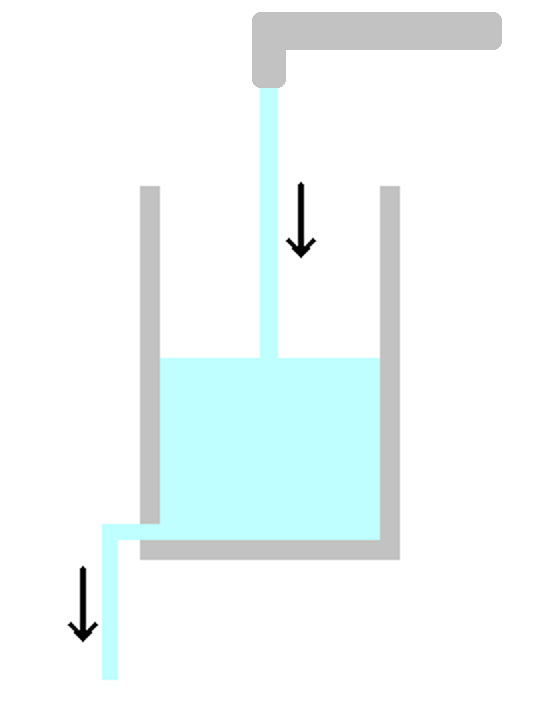
\includegraphics[height=6cm]{glass.png}
  \end{center}
\end{frame}


\begin{frame}{A neuron}
  \begin{center}
    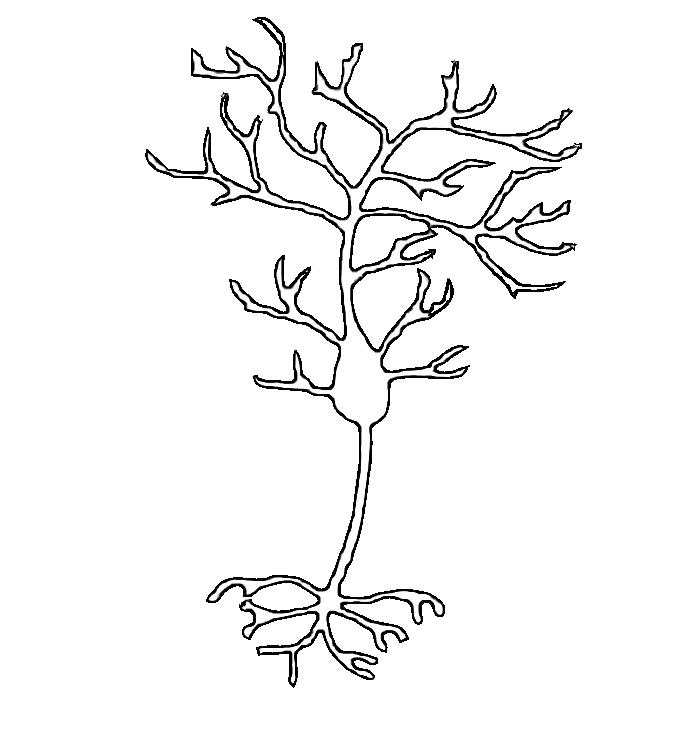
\includegraphics[height=8cm]{neuron.png}
  \end{center}
\end{frame}

\begin{frame}{A neuron has an inside and an outside}
  \begin{center}
    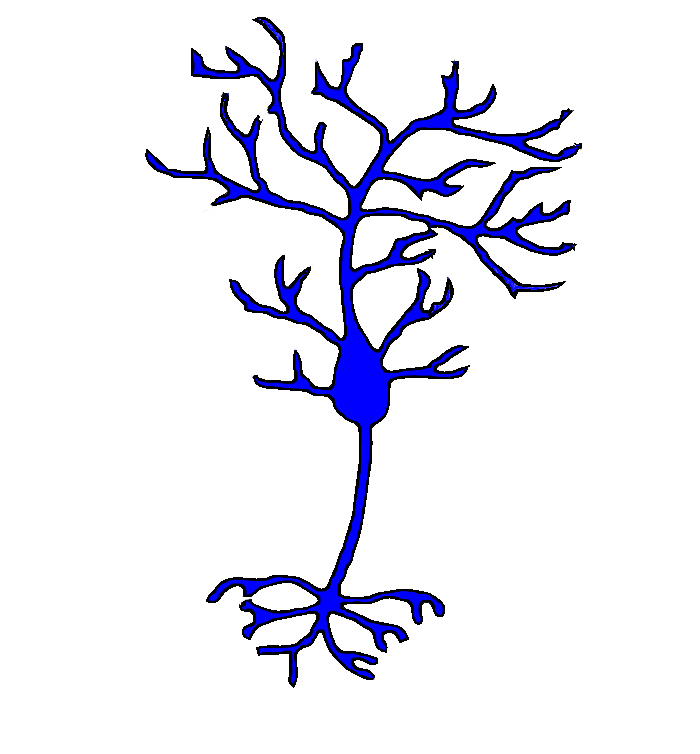
\includegraphics[height=8cm]{neuron_filled.png}
  \end{center}
\end{frame}

\begin{frame}{A neuron has an inside and an outside}
  \begin{center}
    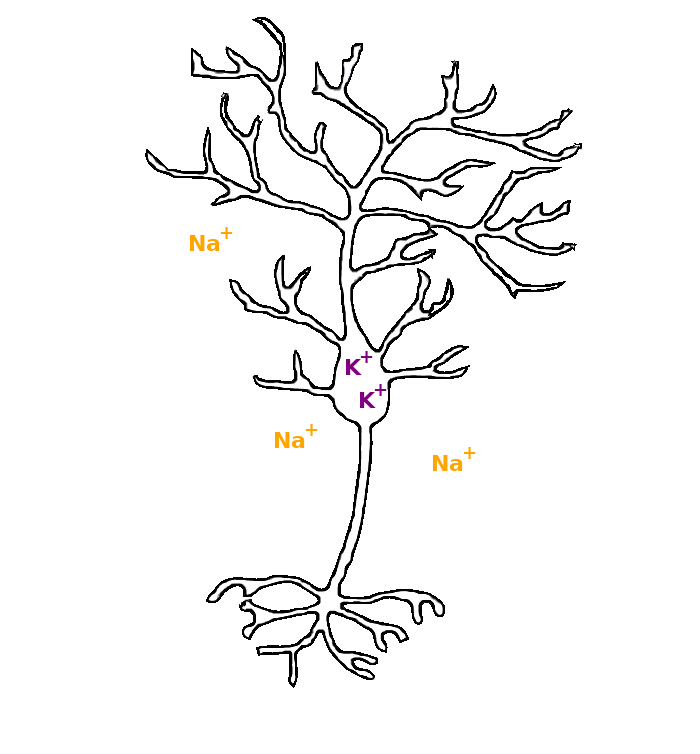
\includegraphics[height=8cm]{ions.png}
  \end{center}
\end{frame}


\begin{frame}{Ion pumps}
  \begin{center}
    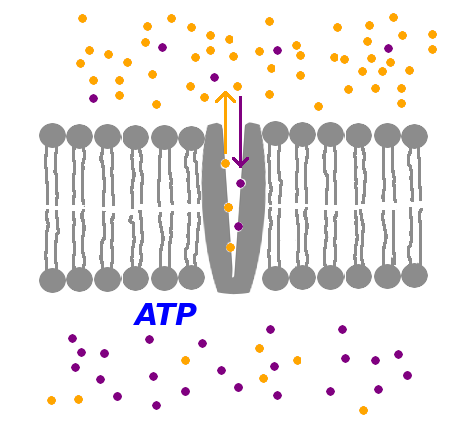
\includegraphics[height=8cm]{ion_pump_1.png}
  \end{center}
\end{frame}


\begin{frame}{Ion pumps}
  \begin{center}
    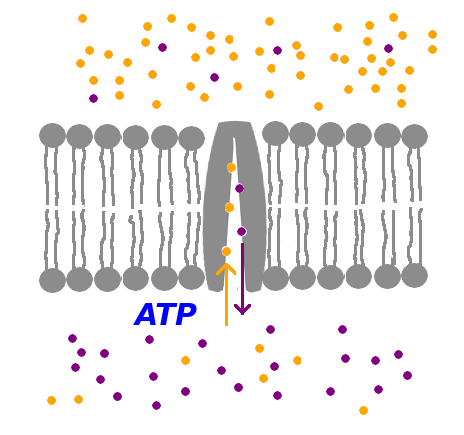
\includegraphics[height=8cm]{ion_pump_2.png}
  \end{center}
\end{frame}


\begin{frame}{Potassium inside and sodium outside}
  \begin{center}
    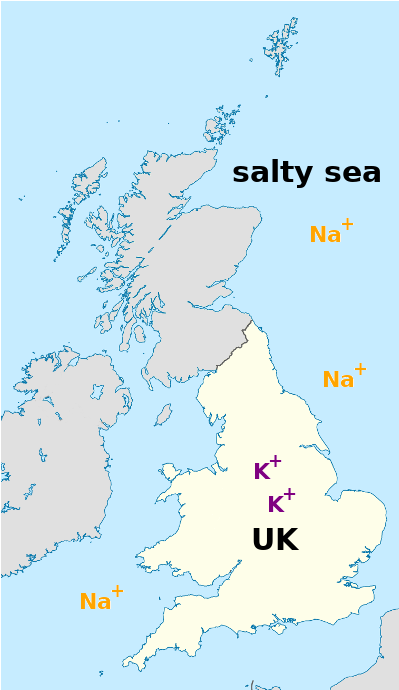
\includegraphics[height=8cm]{uk.png}
  \end{center}
\end{frame}

\begin{frame}{Ions can get through the membrane}
  \begin{center}
    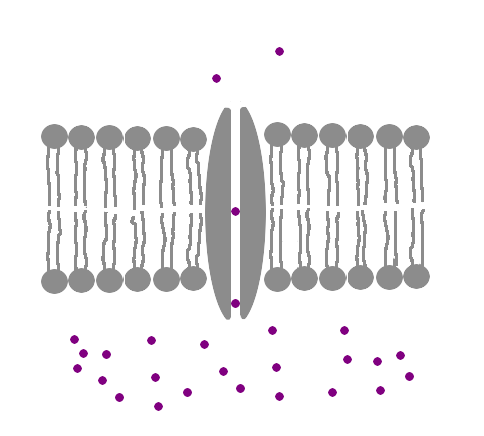
\includegraphics[height=6cm]{passive_channel.png}
  \end{center}
\end{frame}

\begin{frame}{Charge is like water}
  \begin{center}
    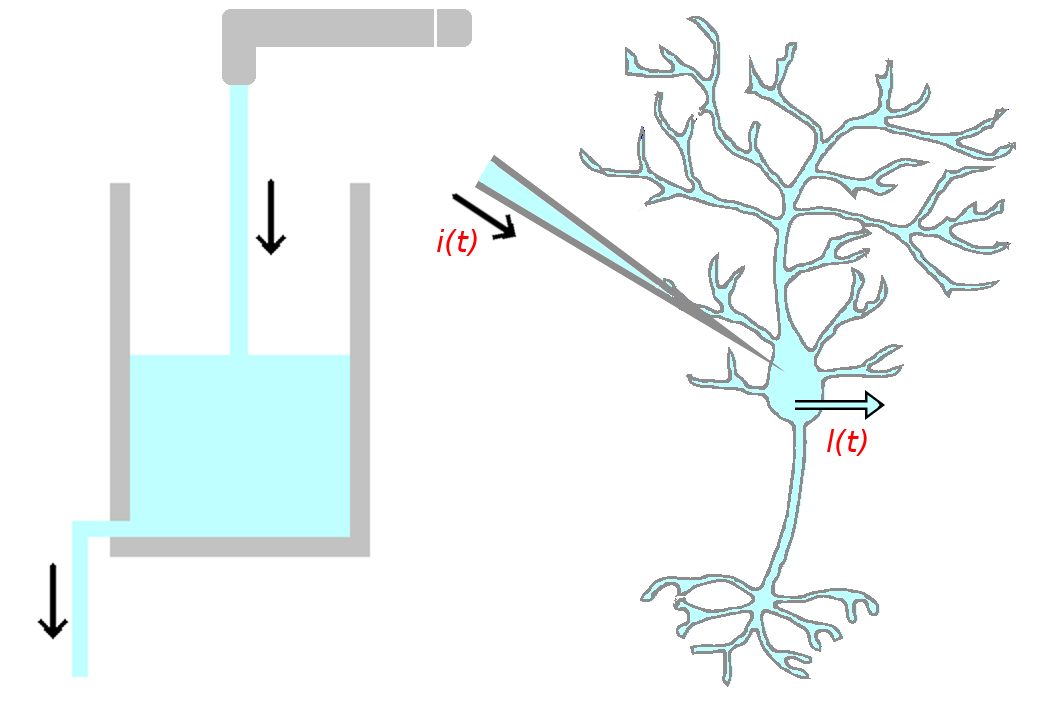
\includegraphics[height=8cm]{glass_neuron.png}
  \end{center}
\end{frame}


\begin{frame}{Voltage difference}
  \begin{columns}
        \begin{column}{0.2\textwidth}
      \end{column}
    \begin{column}{0.3\textwidth}
  $\cred V\crish\sim -70\mbox{mV}\cbla $
    \end{column}
    \begin{column}{0.3\textwidth}
    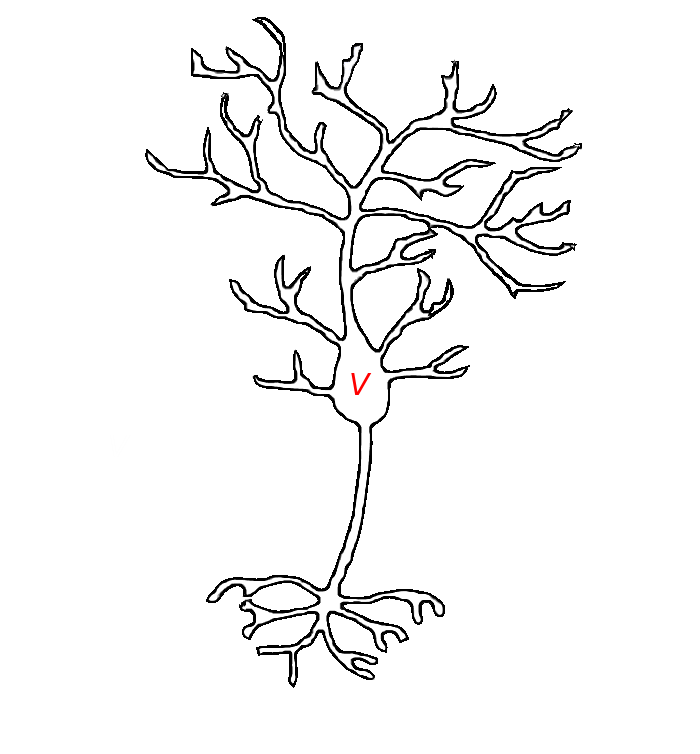
\includegraphics[height=8cm]{voltage.png}
    \end{column}
    \begin{column}{0.2\textwidth}
      \end{column}
    \end{columns}
\end{frame}

\begin{frame}{Voltage is like pressure}
  \begin{quote}
   \textbf{Voltage} is defined as the work needed per unit of charge to move a
    test charge between the two points.
  \end{quote}
\end{frame}


\begin{frame}{Capacitance}
\crish
$$Q=CV$$
\cbla  
\end{frame}


\begin{frame}{Ohm's law}
\crish
$$V=IR$$
\cbla
\begin{center}
    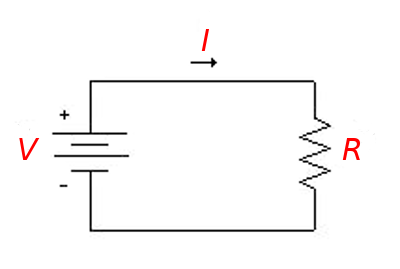
\includegraphics[height=5cm]{basic_circuit.png}
\end{center}
\end{frame}


\begin{frame}{Resistance versus Conductance}
\crish
$$G=1/R$$
\cbla{}so\crish
$$I=GV$$
\cbla
\begin{center}
    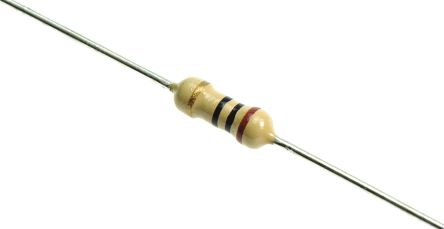
\includegraphics[height=5cm]{resistor.jpg}
\end{center}
\end{frame}


\begin{frame}{Voltage and current}
\crish
$$I=GV$$
\cbla{}so\crish{} $V=0$\cbla{} means \crish{} $I=0$\cbla{}.
\begin{center}
    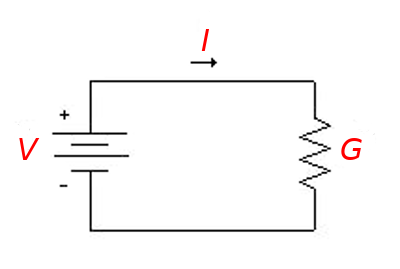
\includegraphics[height=5cm]{basic_circuit_g.png}
\end{center}
\end{frame}

\begin{frame}{Chemical gradients}
\begin{center}
    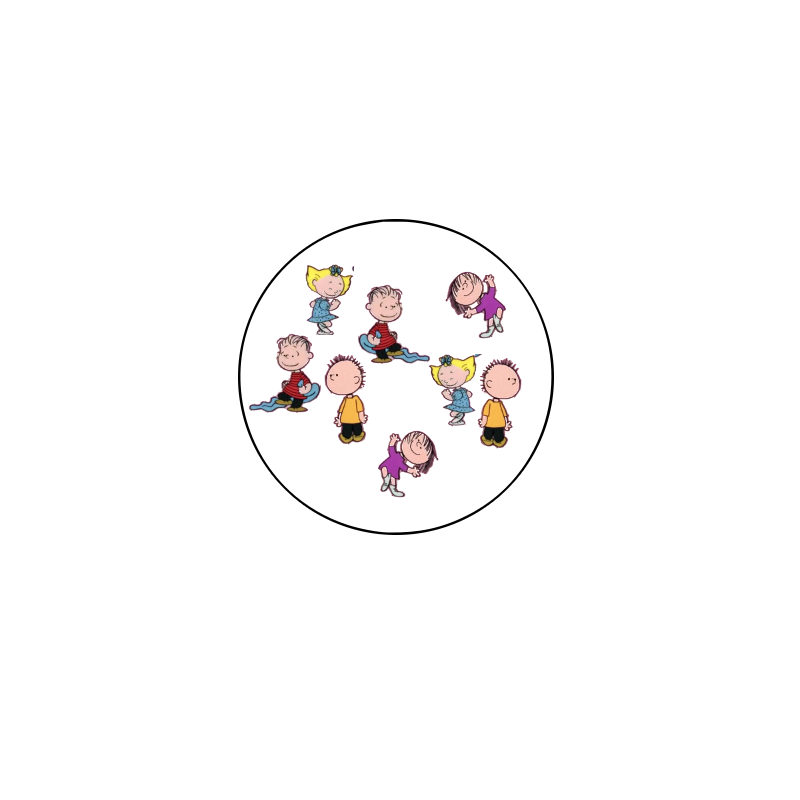
\includegraphics[height=8cm]{children1.png}
\end{center}
\end{frame}

\begin{frame}{Chemical gradients}
\begin{center}
    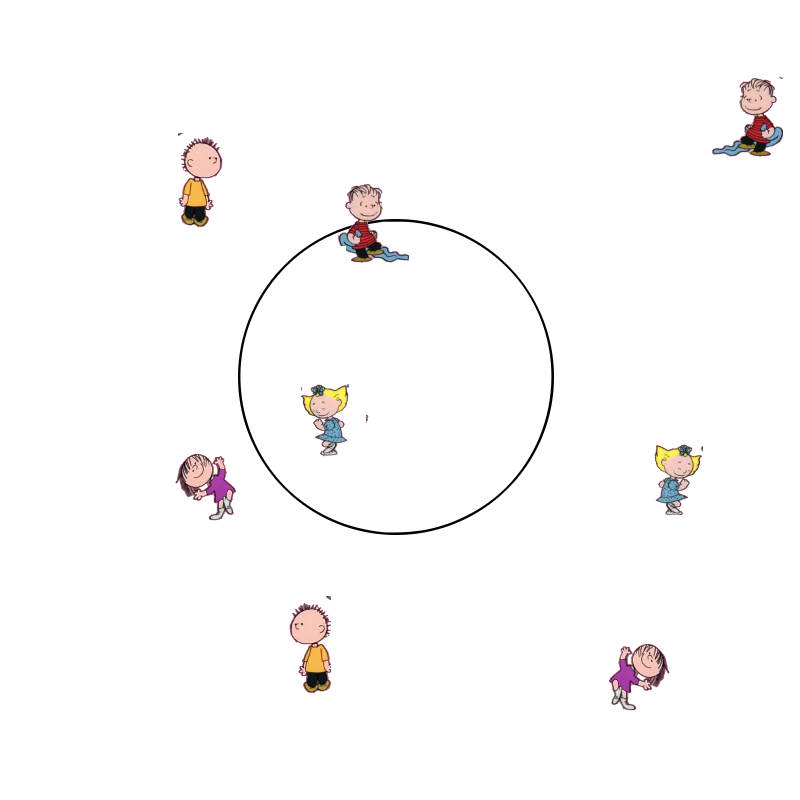
\includegraphics[height=8cm]{children2.png}
\end{center}
\end{frame}

\begin{frame}{Chemical gradients}
\begin{center}
    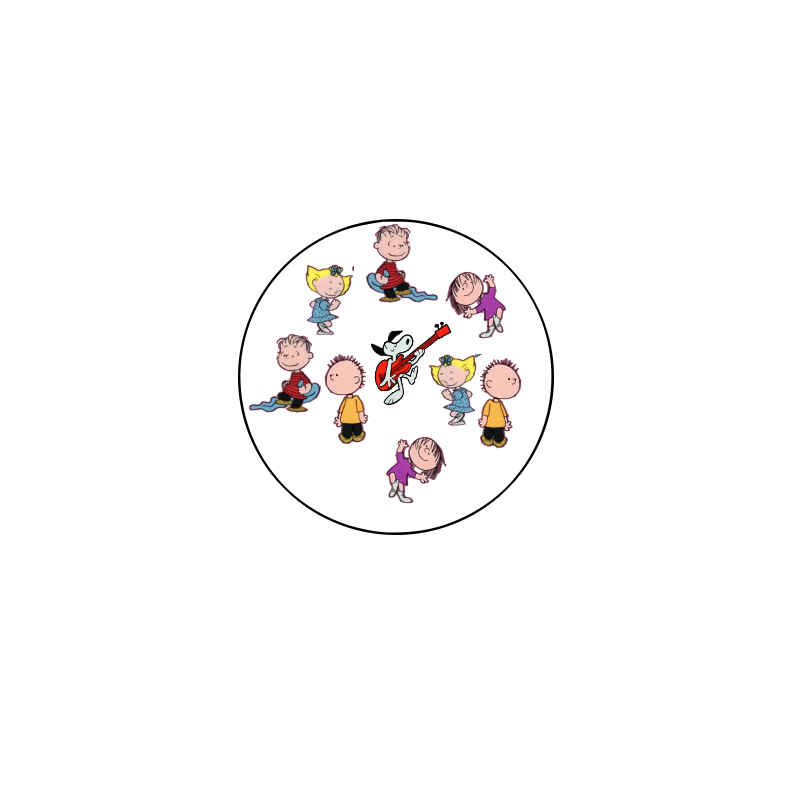
\includegraphics[height=8cm]{children3.png}
\end{center}
\end{frame}

\begin{frame}{Chemical gradients}
\begin{center}
    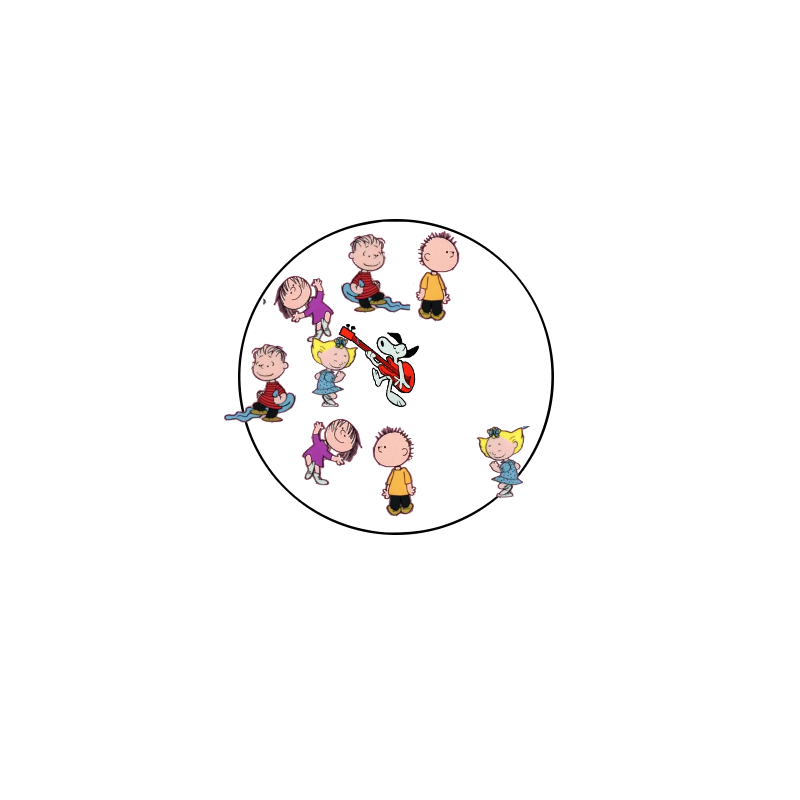
\includegraphics[height=8cm]{children4.png}
\end{center}
\end{frame}

\begin{frame}{Chemical gradients}
  \begin{center}
    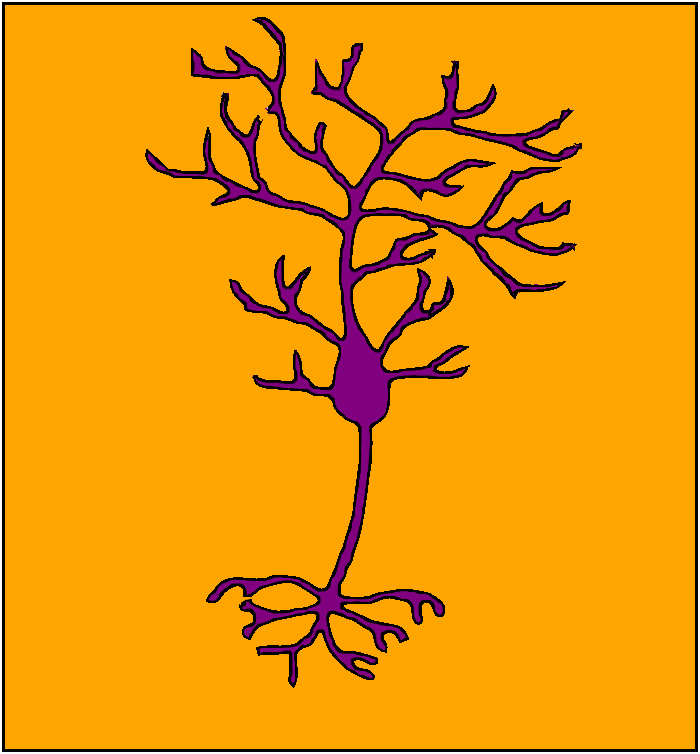
\includegraphics[height=8cm]{neuron_ions.png}
  \end{center}
\end{frame}


\begin{frame}{Chemical gradients}
  \begin{center}
    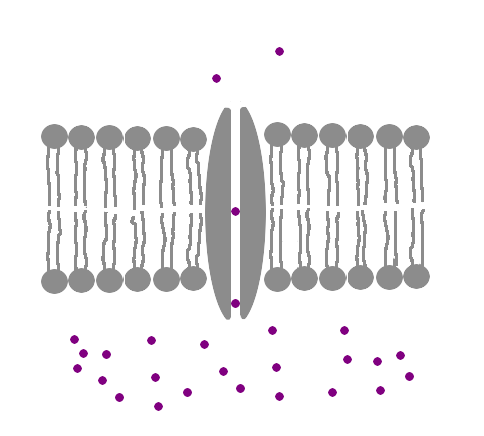
\includegraphics[height=6cm]{passive_channel.png}
  \end{center}
\end{frame}


\begin{frame}{Leak potential}
  \crish
  $$I_l=G(\cred{}E_l\crish{}-V)$$
\cbla{}
  where \cred$E_l\sim -70$mV\cbla{} is the \cblu{}leak reversal potential\cbla{}. 
\end{frame}


\begin{frame}{Leak potential}
  \crish
  $$I_l=G(E_l-V)$$
\cbla{}

DON'T WORRY TO MUCH ABOUT THE SIGN, it is easy to get confused so I
WILL MAKE SURE IT IS RIGHT, this is the expression for the current
inward.
\end{frame}



\begin{frame}{Leak conductance}
  \crish
  $$I_l=\cred{}G\crish{}(E_l-V)$$

  \cbla{} The conductance \cred$G$\cbla{} is the conductance of the membrane and is often called the \cblu{}leak conductance\cbla{}, in fact, there are other conductance that depend on \crish$V$\cbla{}, whereas the leak conductance is constant and sometimes called \cblu{}passive\cbla{}. The symbol \cred{}$g_l$\cbla{} is often used:

  \crish
  $$I_l=g_l(E_l-V)$$
\cbla{}
\end{frame}

\begin{frame}{The leaky integrator for neurons}
\begin{quote}
  rate of change of charge = current in - leak out
\end{quote}
\end{frame}

\begin{frame}{The leaky integrator for neurons}
  \crish
  $$\frac{dQ}{dt}=i(t)-I_l(t)$$
  \cbla
\end{frame}

\begin{frame}{Input}
  For now imagine the input is from an electrode, the electrode input is written:\crish
  $$i(t)=I_e(t)$$
  \cbla
\end{frame}

\begin{frame}{The leaky integrator for neurons}
  \crish
  $$C\frac{dV}{dt}=g_l(E_l-V)+I_e(t)$$
  \cbla
\end{frame}


\begin{frame}{The leaky integrator for neurons}
Dividing across by the \crish{}$g_l$\cbla{} we get
  \crish
  $$\tau_m\frac{dV}{dt}=E_l-V+R_mI_e(t)$$
  \cbla
  where \crish$\tau_m$\cbla{} is called the \cblu{}membrane time constant\cbla{} and \crish{}$R_m=1/g_l$\cbla{} is called the \cblu{}the membrane resistance\cbla{}.

\end{frame}



\begin{frame}{The leaky bucket redux}

  \crish
  $$\tau_m\frac{dV}{dt}=E_l-V+R_mI_e(t)$$
  \cbla

  We have seen more-or-less this equation before, all that is really
  different is the extra constant \crish$E_l$\cbla{} and so know how to
  deal with the equation, for example, if \crish{}$I_e$\cbla{} is constant the
  solution is\crish

  $$V(t)=E_l+R_mI_e+[V(0)-E_l-R_mI_e]e^{-t/\tau_m}$$
  \cbla{}
  
\end{frame}

\begin{frame}{Voltage gated channels}
  This isn't the full story
  \crish$$\tau_m\frac{dV}{dt}=E_l-V+R_mI_e(t)+R_m(\cred{}\mbox{currents from the gated channels}\crish)$$\cbla{}
  \begin{center}
    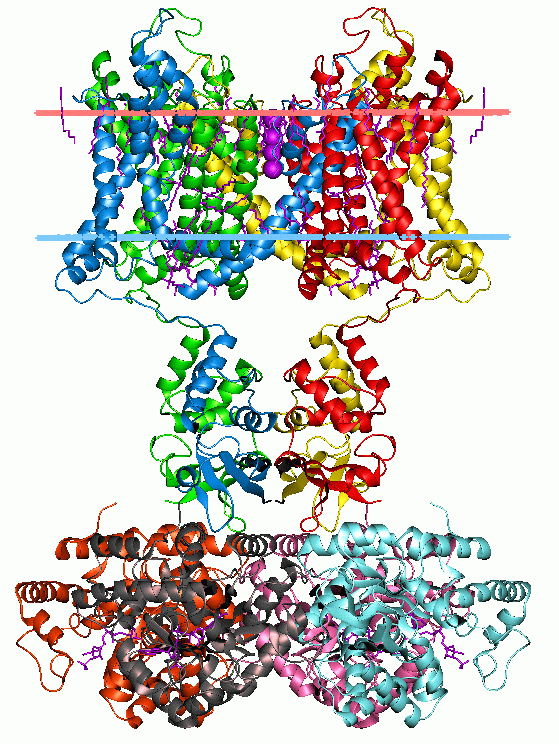
\includegraphics[height=4cm]{2r9r_opm.png}
\end{center}
    \vfill
  \flushright{\tiny{image from wikipedia}}
  \end{frame}


\begin{frame}{Action potential}
  \begin{center}
    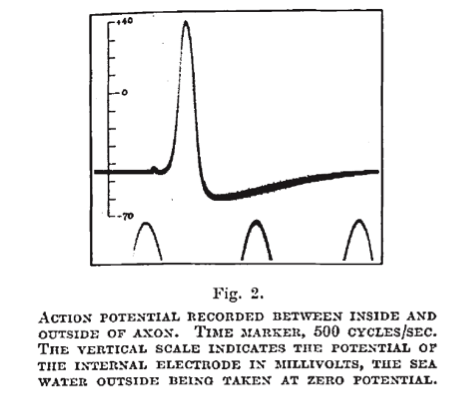
\includegraphics[height=8cm]{HH_spike.png}
\end{center}
    \vfill
  \flushright{\tiny{image from Hodgkin and Huxley}}
  \end{frame}

\begin{frame}{Leaky integrate and fire model}

  \crish
  $$\tau_m\frac{dV}{dt}=E_l-V+R_mI_e(t)$$
  \cbla

and put the spike in `by hand'!
  
\end{frame}


\begin{frame}{Leaky integrate and fire model}

  \crish
  $$\tau_m\frac{dV}{dt}=E_l-V+R_mI_e(t)$$
  \cbla

  if \crish{}$V>V_T$\cbla{} there is a \cblu{}spike\cbla{} and \crish{}$V=V_R$\cbla{}.
  
\end{frame}


\begin{frame}{Leaky integrate and fire model}

  \crish
  $$\tau_m\frac{dV}{dt}=E_l-V+R_mI_e(t)$$
  \cbla

  we call \crish{}$V_T $\cbla{} the \cblu{}threshold\cbla{} and
  \crish{}$V_R$\cbla the \cblu{} reset\cbla{}.
  
\end{frame}


\begin{frame}{Leaky integrate and fire model}

  \crish
  $$\tau_m\frac{dV}{dt}=E_l-V+R_mI_e(t)$$
  \cbla

  with, for example, \crish{}$V_T\sim-55 $ mV\cbla{} and \crish{}$V_R\sim-70$ mV\cbla.
  
\end{frame}

\begin{frame}{Constant input}

  \crish
  $$\tau_m\frac{dV}{dt}=\bar{V}-V$$
  \cbla{}

  where \crish{}$\bar{V}=E_l+R_mI_e$\cbla{} then\crish{}

  $$V(t)=\bar{V}+[V(0)-\bar{V}]e^{-t/\tau_m}$$
\cbla{}
\end{frame}

\begin{frame}{Constant input}
\crish{}
  $$V(t)=\bar{V}+[V(0)-\bar{V}]e^{-t/\tau_m}$$
\cbla{}

If \crish{}$\bar{V}<V_T$\cbla{} the neuron will never spike!
  
\end{frame}


\begin{frame}{Regular spiking}
  \begin{center}
    % GNUPLOT: LaTeX picture with Postscript
\begingroup
  \makeatletter
  \providecommand\color[2][]{%
    \GenericError{(gnuplot) \space\space\space\@spaces}{%
      Package color not loaded in conjunction with
      terminal option `colourtext'%
    }{See the gnuplot documentation for explanation.%
    }{Either use 'blacktext' in gnuplot or load the package
      color.sty in LaTeX.}%
    \renewcommand\color[2][]{}%
  }%
  \providecommand\includegraphics[2][]{%
    \GenericError{(gnuplot) \space\space\space\@spaces}{%
      Package graphicx or graphics not loaded%
    }{See the gnuplot documentation for explanation.%
    }{The gnuplot epslatex terminal needs graphicx.sty or graphics.sty.}%
    \renewcommand\includegraphics[2][]{}%
  }%
  \providecommand\rotatebox[2]{#2}%
  \@ifundefined{ifGPcolor}{%
    \newif\ifGPcolor
    \GPcolorfalse
  }{}%
  \@ifundefined{ifGPblacktext}{%
    \newif\ifGPblacktext
    \GPblacktexttrue
  }{}%
  % define a \g@addto@macro without @ in the name:
  \let\gplgaddtomacro\g@addto@macro
  % define empty templates for all commands taking text:
  \gdef\gplbacktext{}%
  \gdef\gplfronttext{}%
  \makeatother
  \ifGPblacktext
    % no textcolor at all
    \def\colorrgb#1{}%
    \def\colorgray#1{}%
  \else
    % gray or color?
    \ifGPcolor
      \def\colorrgb#1{\color[rgb]{#1}}%
      \def\colorgray#1{\color[gray]{#1}}%
      \expandafter\def\csname LTw\endcsname{\color{white}}%
      \expandafter\def\csname LTb\endcsname{\color{black}}%
      \expandafter\def\csname LTa\endcsname{\color{black}}%
      \expandafter\def\csname LT0\endcsname{\color[rgb]{1,0,0}}%
      \expandafter\def\csname LT1\endcsname{\color[rgb]{0,1,0}}%
      \expandafter\def\csname LT2\endcsname{\color[rgb]{0,0,1}}%
      \expandafter\def\csname LT3\endcsname{\color[rgb]{1,0,1}}%
      \expandafter\def\csname LT4\endcsname{\color[rgb]{0,1,1}}%
      \expandafter\def\csname LT5\endcsname{\color[rgb]{1,1,0}}%
      \expandafter\def\csname LT6\endcsname{\color[rgb]{0,0,0}}%
      \expandafter\def\csname LT7\endcsname{\color[rgb]{1,0.3,0}}%
      \expandafter\def\csname LT8\endcsname{\color[rgb]{0.5,0.5,0.5}}%
    \else
      % gray
      \def\colorrgb#1{\color{black}}%
      \def\colorgray#1{\color[gray]{#1}}%
      \expandafter\def\csname LTw\endcsname{\color{white}}%
      \expandafter\def\csname LTb\endcsname{\color{black}}%
      \expandafter\def\csname LTa\endcsname{\color{black}}%
      \expandafter\def\csname LT0\endcsname{\color{black}}%
      \expandafter\def\csname LT1\endcsname{\color{black}}%
      \expandafter\def\csname LT2\endcsname{\color{black}}%
      \expandafter\def\csname LT3\endcsname{\color{black}}%
      \expandafter\def\csname LT4\endcsname{\color{black}}%
      \expandafter\def\csname LT5\endcsname{\color{black}}%
      \expandafter\def\csname LT6\endcsname{\color{black}}%
      \expandafter\def\csname LT7\endcsname{\color{black}}%
      \expandafter\def\csname LT8\endcsname{\color{black}}%
    \fi
  \fi
  \setlength{\unitlength}{0.0500bp}%
  \begin{picture}(5760.00,4032.00)%
    \gplgaddtomacro\gplbacktext{%
      \csname LTb\endcsname%
      \put(814,996){\makebox(0,0)[r]{\strut{}-70}}%
      \put(814,1433){\makebox(0,0)[r]{\strut{}-55}}%
      \put(814,3038){\makebox(0,0)[r]{\strut{} 0}}%
      \put(814,3621){\makebox(0,0)[r]{\strut{} 20}}%
      \put(946,484){\makebox(0,0){\strut{} 0}}%
      \put(1829,484){\makebox(0,0){\strut{} 20}}%
      \put(2713,484){\makebox(0,0){\strut{} 40}}%
      \put(3596,484){\makebox(0,0){\strut{} 60}}%
      \put(4480,484){\makebox(0,0){\strut{} 80}}%
      \put(5363,484){\makebox(0,0){\strut{} 100}}%
      \put(176,2235){\rotatebox{-270}{\makebox(0,0){\strut{}$V$ (mV)}}}%
      \put(3154,154){\makebox(0,0){\strut{}$t$ (ms)}}%
    }%
    \gplgaddtomacro\gplfronttext{%
      \csname LTb\endcsname%
      \put(2662,3594){\makebox(0,0)[r]{\strut{}$R_mI_e = 12$ mV}}%
    }%
    \gplbacktext
    \put(0,0){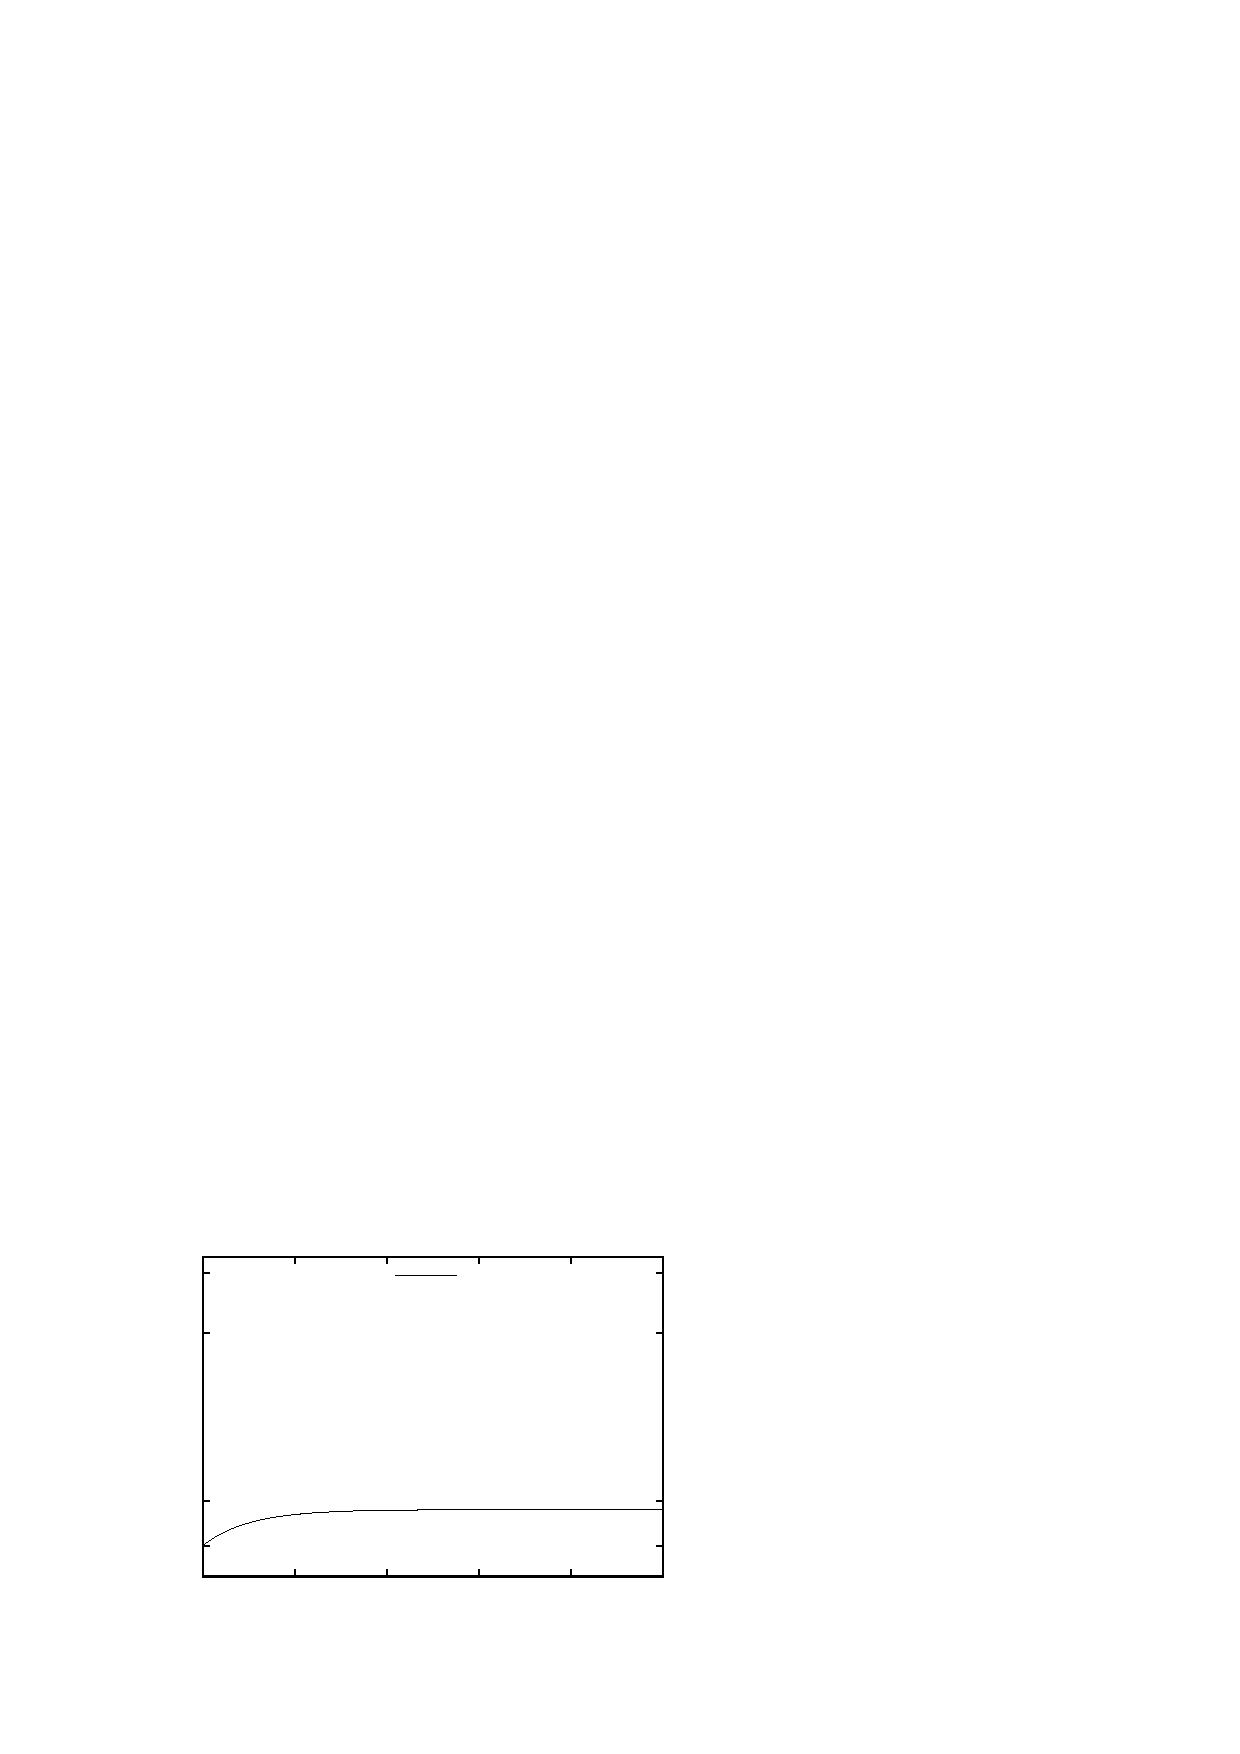
\includegraphics{v_i_f_no}}%
    \gplfronttext
  \end{picture}%
\endgroup

\end{center}
  \end{frame}



\begin{frame}{Constant input}
\crish{}
  $$V(t)=\bar{V}+[V(0)-\bar{V}]e^{-t/\tau_m}$$
\cbla{}

If \crish{}$\bar{V}>V_T$\cbla{} it will approach \crish{}$\bar{V}$\cbla{} but reach \crish{}$V_T$\cbla{} on the way and spike.
  
\end{frame}


\begin{frame}{Regular spiking}
  \begin{center}
    % GNUPLOT: LaTeX picture with Postscript
\begingroup
  \makeatletter
  \providecommand\color[2][]{%
    \GenericError{(gnuplot) \space\space\space\@spaces}{%
      Package color not loaded in conjunction with
      terminal option `colourtext'%
    }{See the gnuplot documentation for explanation.%
    }{Either use 'blacktext' in gnuplot or load the package
      color.sty in LaTeX.}%
    \renewcommand\color[2][]{}%
  }%
  \providecommand\includegraphics[2][]{%
    \GenericError{(gnuplot) \space\space\space\@spaces}{%
      Package graphicx or graphics not loaded%
    }{See the gnuplot documentation for explanation.%
    }{The gnuplot epslatex terminal needs graphicx.sty or graphics.sty.}%
    \renewcommand\includegraphics[2][]{}%
  }%
  \providecommand\rotatebox[2]{#2}%
  \@ifundefined{ifGPcolor}{%
    \newif\ifGPcolor
    \GPcolorfalse
  }{}%
  \@ifundefined{ifGPblacktext}{%
    \newif\ifGPblacktext
    \GPblacktexttrue
  }{}%
  % define a \g@addto@macro without @ in the name:
  \let\gplgaddtomacro\g@addto@macro
  % define empty templates for all commands taking text:
  \gdef\gplbacktext{}%
  \gdef\gplfronttext{}%
  \makeatother
  \ifGPblacktext
    % no textcolor at all
    \def\colorrgb#1{}%
    \def\colorgray#1{}%
  \else
    % gray or color?
    \ifGPcolor
      \def\colorrgb#1{\color[rgb]{#1}}%
      \def\colorgray#1{\color[gray]{#1}}%
      \expandafter\def\csname LTw\endcsname{\color{white}}%
      \expandafter\def\csname LTb\endcsname{\color{black}}%
      \expandafter\def\csname LTa\endcsname{\color{black}}%
      \expandafter\def\csname LT0\endcsname{\color[rgb]{1,0,0}}%
      \expandafter\def\csname LT1\endcsname{\color[rgb]{0,1,0}}%
      \expandafter\def\csname LT2\endcsname{\color[rgb]{0,0,1}}%
      \expandafter\def\csname LT3\endcsname{\color[rgb]{1,0,1}}%
      \expandafter\def\csname LT4\endcsname{\color[rgb]{0,1,1}}%
      \expandafter\def\csname LT5\endcsname{\color[rgb]{1,1,0}}%
      \expandafter\def\csname LT6\endcsname{\color[rgb]{0,0,0}}%
      \expandafter\def\csname LT7\endcsname{\color[rgb]{1,0.3,0}}%
      \expandafter\def\csname LT8\endcsname{\color[rgb]{0.5,0.5,0.5}}%
    \else
      % gray
      \def\colorrgb#1{\color{black}}%
      \def\colorgray#1{\color[gray]{#1}}%
      \expandafter\def\csname LTw\endcsname{\color{white}}%
      \expandafter\def\csname LTb\endcsname{\color{black}}%
      \expandafter\def\csname LTa\endcsname{\color{black}}%
      \expandafter\def\csname LT0\endcsname{\color{black}}%
      \expandafter\def\csname LT1\endcsname{\color{black}}%
      \expandafter\def\csname LT2\endcsname{\color{black}}%
      \expandafter\def\csname LT3\endcsname{\color{black}}%
      \expandafter\def\csname LT4\endcsname{\color{black}}%
      \expandafter\def\csname LT5\endcsname{\color{black}}%
      \expandafter\def\csname LT6\endcsname{\color{black}}%
      \expandafter\def\csname LT7\endcsname{\color{black}}%
      \expandafter\def\csname LT8\endcsname{\color{black}}%
    \fi
  \fi
  \setlength{\unitlength}{0.0500bp}%
  \begin{picture}(7200.00,5040.00)%
    \gplgaddtomacro\gplbacktext{%
      \csname LTb\endcsname%
      \put(594,440){\makebox(0,0)[r]{\strut{}-70}}%
      \put(594,922){\makebox(0,0)[r]{\strut{}-60}}%
      \put(594,1403){\makebox(0,0)[r]{\strut{}-50}}%
      \put(594,1885){\makebox(0,0)[r]{\strut{}-40}}%
      \put(594,2367){\makebox(0,0)[r]{\strut{}-30}}%
      \put(594,2848){\makebox(0,0)[r]{\strut{}-20}}%
      \put(594,3330){\makebox(0,0)[r]{\strut{}-10}}%
      \put(594,3812){\makebox(0,0)[r]{\strut{} 0}}%
      \put(594,4293){\makebox(0,0)[r]{\strut{} 10}}%
      \put(594,4775){\makebox(0,0)[r]{\strut{} 20}}%
      \put(726,220){\makebox(0,0){\strut{} 0}}%
      \put(1941,220){\makebox(0,0){\strut{} 20}}%
      \put(3157,220){\makebox(0,0){\strut{} 40}}%
      \put(4372,220){\makebox(0,0){\strut{} 60}}%
      \put(5588,220){\makebox(0,0){\strut{} 80}}%
      \put(6803,220){\makebox(0,0){\strut{} 100}}%
    }%
    \gplgaddtomacro\gplfronttext{%
      \csname LTb\endcsname%
      \put(2178,4602){\makebox(0,0)[r]{\strut{} $R_mI_e=16$ mV}}%
      \csname LTb\endcsname%
      \put(2178,4382){\makebox(0,0)[r]{\strut{} $R_mI_e=12$ mV}}%
      \put(4000,0){\makebox(0,0)[r]{\strut{} $t$ (ms)}}%
      \put(0,3000){\makebox(0,0)[r]{\strut{} $V$ (mV)}}%
    }%
    \gplbacktext
    \put(0,0){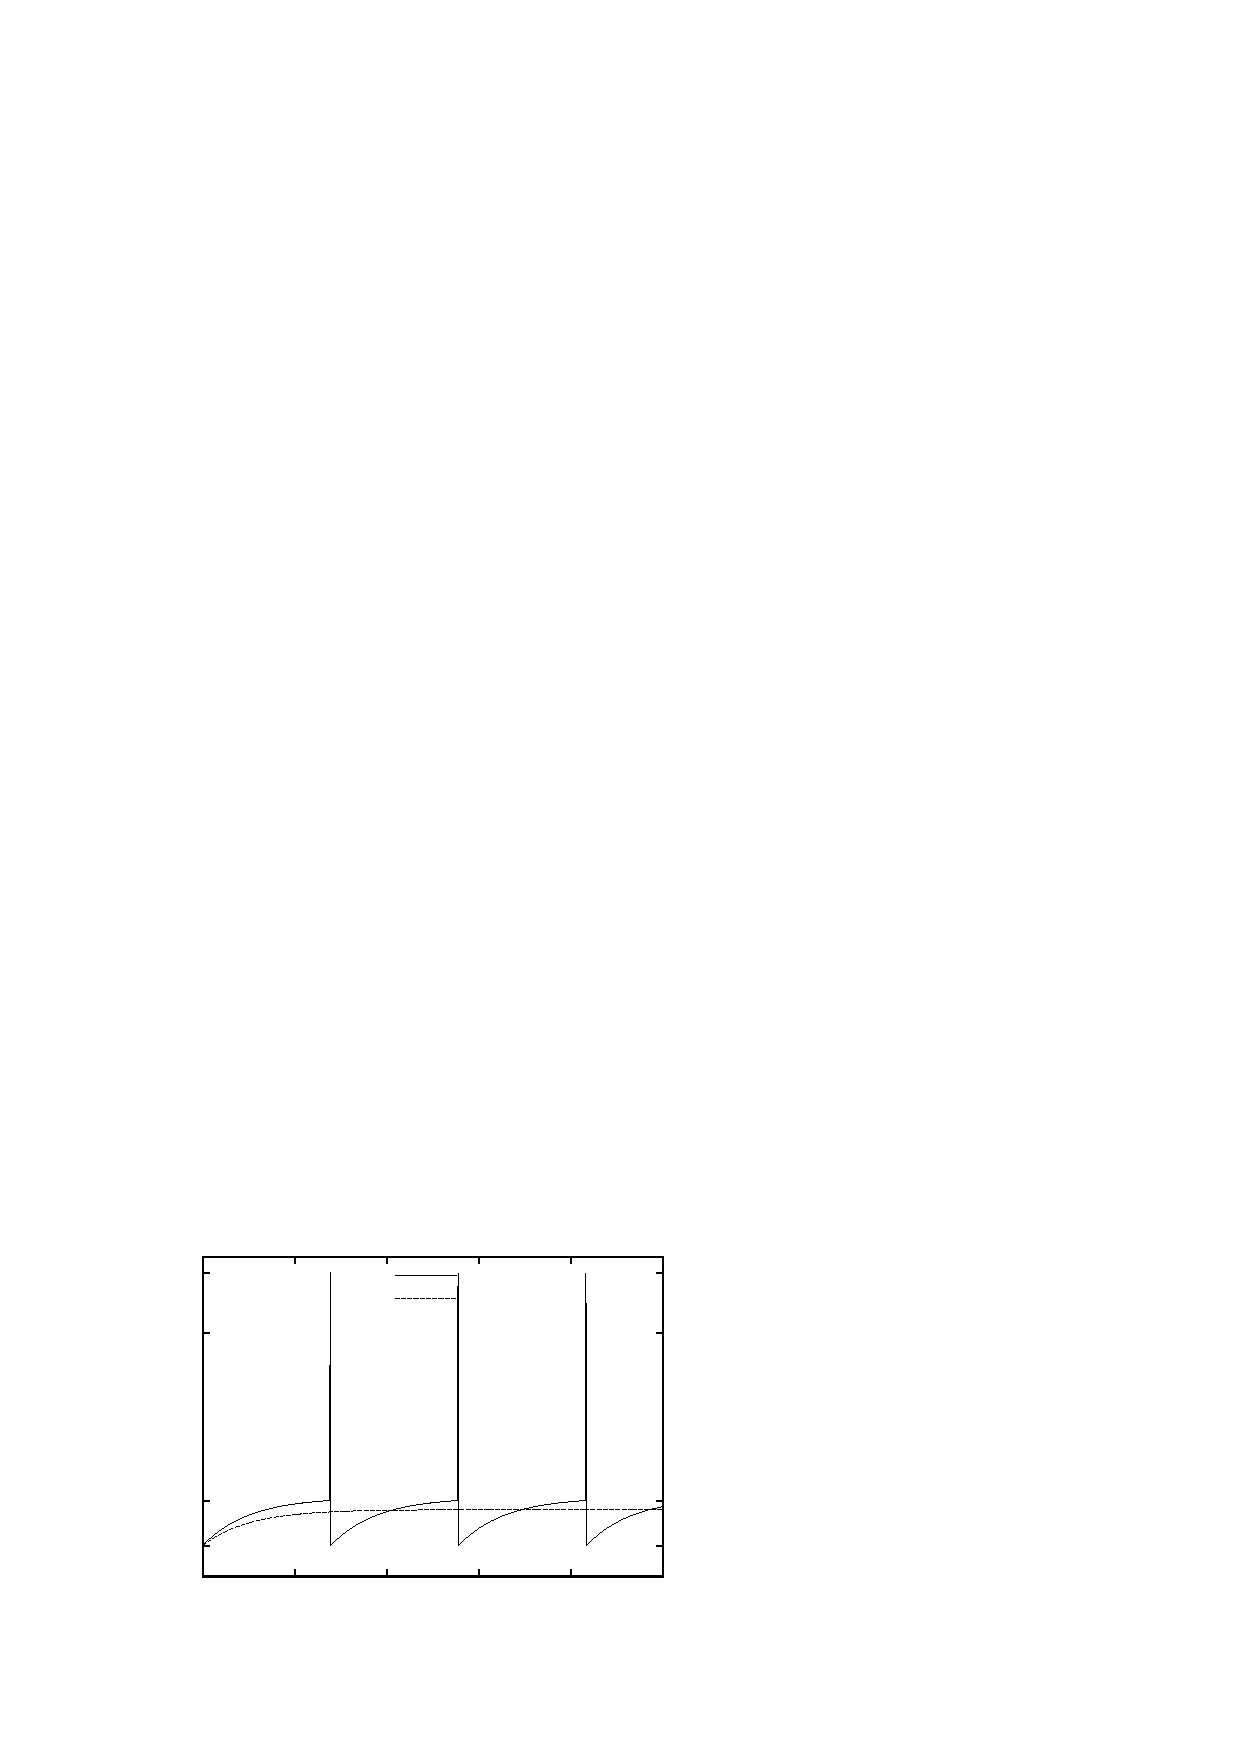
\includegraphics{v_i_f}}%
    \gplfronttext
  \end{picture}%
\endgroup

\end{center}
  \end{frame}

\begin{frame}{f-I curve}
  \begin{center}
    % GNUPLOT: LaTeX picture with Postscript
\begingroup
  \makeatletter
  \providecommand\color[2][]{%
    \GenericError{(gnuplot) \space\space\space\@spaces}{%
      Package color not loaded in conjunction with
      terminal option `colourtext'%
    }{See the gnuplot documentation for explanation.%
    }{Either use 'blacktext' in gnuplot or load the package
      color.sty in LaTeX.}%
    \renewcommand\color[2][]{}%
  }%
  \providecommand\includegraphics[2][]{%
    \GenericError{(gnuplot) \space\space\space\@spaces}{%
      Package graphicx or graphics not loaded%
    }{See the gnuplot documentation for explanation.%
    }{The gnuplot epslatex terminal needs graphicx.sty or graphics.sty.}%
    \renewcommand\includegraphics[2][]{}%
  }%
  \providecommand\rotatebox[2]{#2}%
  \@ifundefined{ifGPcolor}{%
    \newif\ifGPcolor
    \GPcolorfalse
  }{}%
  \@ifundefined{ifGPblacktext}{%
    \newif\ifGPblacktext
    \GPblacktexttrue
  }{}%
  % define a \g@addto@macro without @ in the name:
  \let\gplgaddtomacro\g@addto@macro
  % define empty templates for all commands taking text:
  \gdef\gplbacktext{}%
  \gdef\gplfronttext{}%
  \makeatother
  \ifGPblacktext
    % no textcolor at all
    \def\colorrgb#1{}%
    \def\colorgray#1{}%
  \else
    % gray or color?
    \ifGPcolor
      \def\colorrgb#1{\color[rgb]{#1}}%
      \def\colorgray#1{\color[gray]{#1}}%
      \expandafter\def\csname LTw\endcsname{\color{white}}%
      \expandafter\def\csname LTb\endcsname{\color{black}}%
      \expandafter\def\csname LTa\endcsname{\color{black}}%
      \expandafter\def\csname LT0\endcsname{\color[rgb]{1,0,0}}%
      \expandafter\def\csname LT1\endcsname{\color[rgb]{0,1,0}}%
      \expandafter\def\csname LT2\endcsname{\color[rgb]{0,0,1}}%
      \expandafter\def\csname LT3\endcsname{\color[rgb]{1,0,1}}%
      \expandafter\def\csname LT4\endcsname{\color[rgb]{0,1,1}}%
      \expandafter\def\csname LT5\endcsname{\color[rgb]{1,1,0}}%
      \expandafter\def\csname LT6\endcsname{\color[rgb]{0,0,0}}%
      \expandafter\def\csname LT7\endcsname{\color[rgb]{1,0.3,0}}%
      \expandafter\def\csname LT8\endcsname{\color[rgb]{0.5,0.5,0.5}}%
    \else
      % gray
      \def\colorrgb#1{\color{black}}%
      \def\colorgray#1{\color[gray]{#1}}%
      \expandafter\def\csname LTw\endcsname{\color{white}}%
      \expandafter\def\csname LTb\endcsname{\color{black}}%
      \expandafter\def\csname LTa\endcsname{\color{black}}%
      \expandafter\def\csname LT0\endcsname{\color{black}}%
      \expandafter\def\csname LT1\endcsname{\color{black}}%
      \expandafter\def\csname LT2\endcsname{\color{black}}%
      \expandafter\def\csname LT3\endcsname{\color{black}}%
      \expandafter\def\csname LT4\endcsname{\color{black}}%
      \expandafter\def\csname LT5\endcsname{\color{black}}%
      \expandafter\def\csname LT6\endcsname{\color{black}}%
      \expandafter\def\csname LT7\endcsname{\color{black}}%
      \expandafter\def\csname LT8\endcsname{\color{black}}%
    \fi
  \fi
  \setlength{\unitlength}{0.0500bp}%
  \begin{picture}(5040.00,3528.00)%
    \gplgaddtomacro\gplbacktext{%
      \csname LTb\endcsname%
      \put(814,704){\makebox(0,0)[r]{\strut{} 0}}%
      \put(814,1024){\makebox(0,0)[r]{\strut{} 10}}%
      \put(814,1344){\makebox(0,0)[r]{\strut{} 20}}%
      \put(814,1664){\makebox(0,0)[r]{\strut{} 30}}%
      \put(814,1984){\makebox(0,0)[r]{\strut{} 40}}%
      \put(814,2303){\makebox(0,0)[r]{\strut{} 50}}%
      \put(814,2623){\makebox(0,0)[r]{\strut{} 60}}%
      \put(814,2943){\makebox(0,0)[r]{\strut{} 70}}%
      \put(814,3263){\makebox(0,0)[r]{\strut{} 80}}%
      \put(946,484){\makebox(0,0){\strut{} 0}}%
      \put(1786,484){\makebox(0,0){\strut{} 5}}%
      \put(2626,484){\makebox(0,0){\strut{} 10}}%
      \put(3467,484){\makebox(0,0){\strut{} 15}}%
      \put(4307,484){\makebox(0,0){\strut{} 20}}%
      \put(176,1983){\rotatebox{-270}{\makebox(0,0){\strut{}firing rate in Hz}}}%
      \put(2794,154){\makebox(0,0){\strut{}$R_mI_e$}}%
    }%
    \gplgaddtomacro\gplfronttext{%
    }%
    \gplbacktext
    \put(0,0){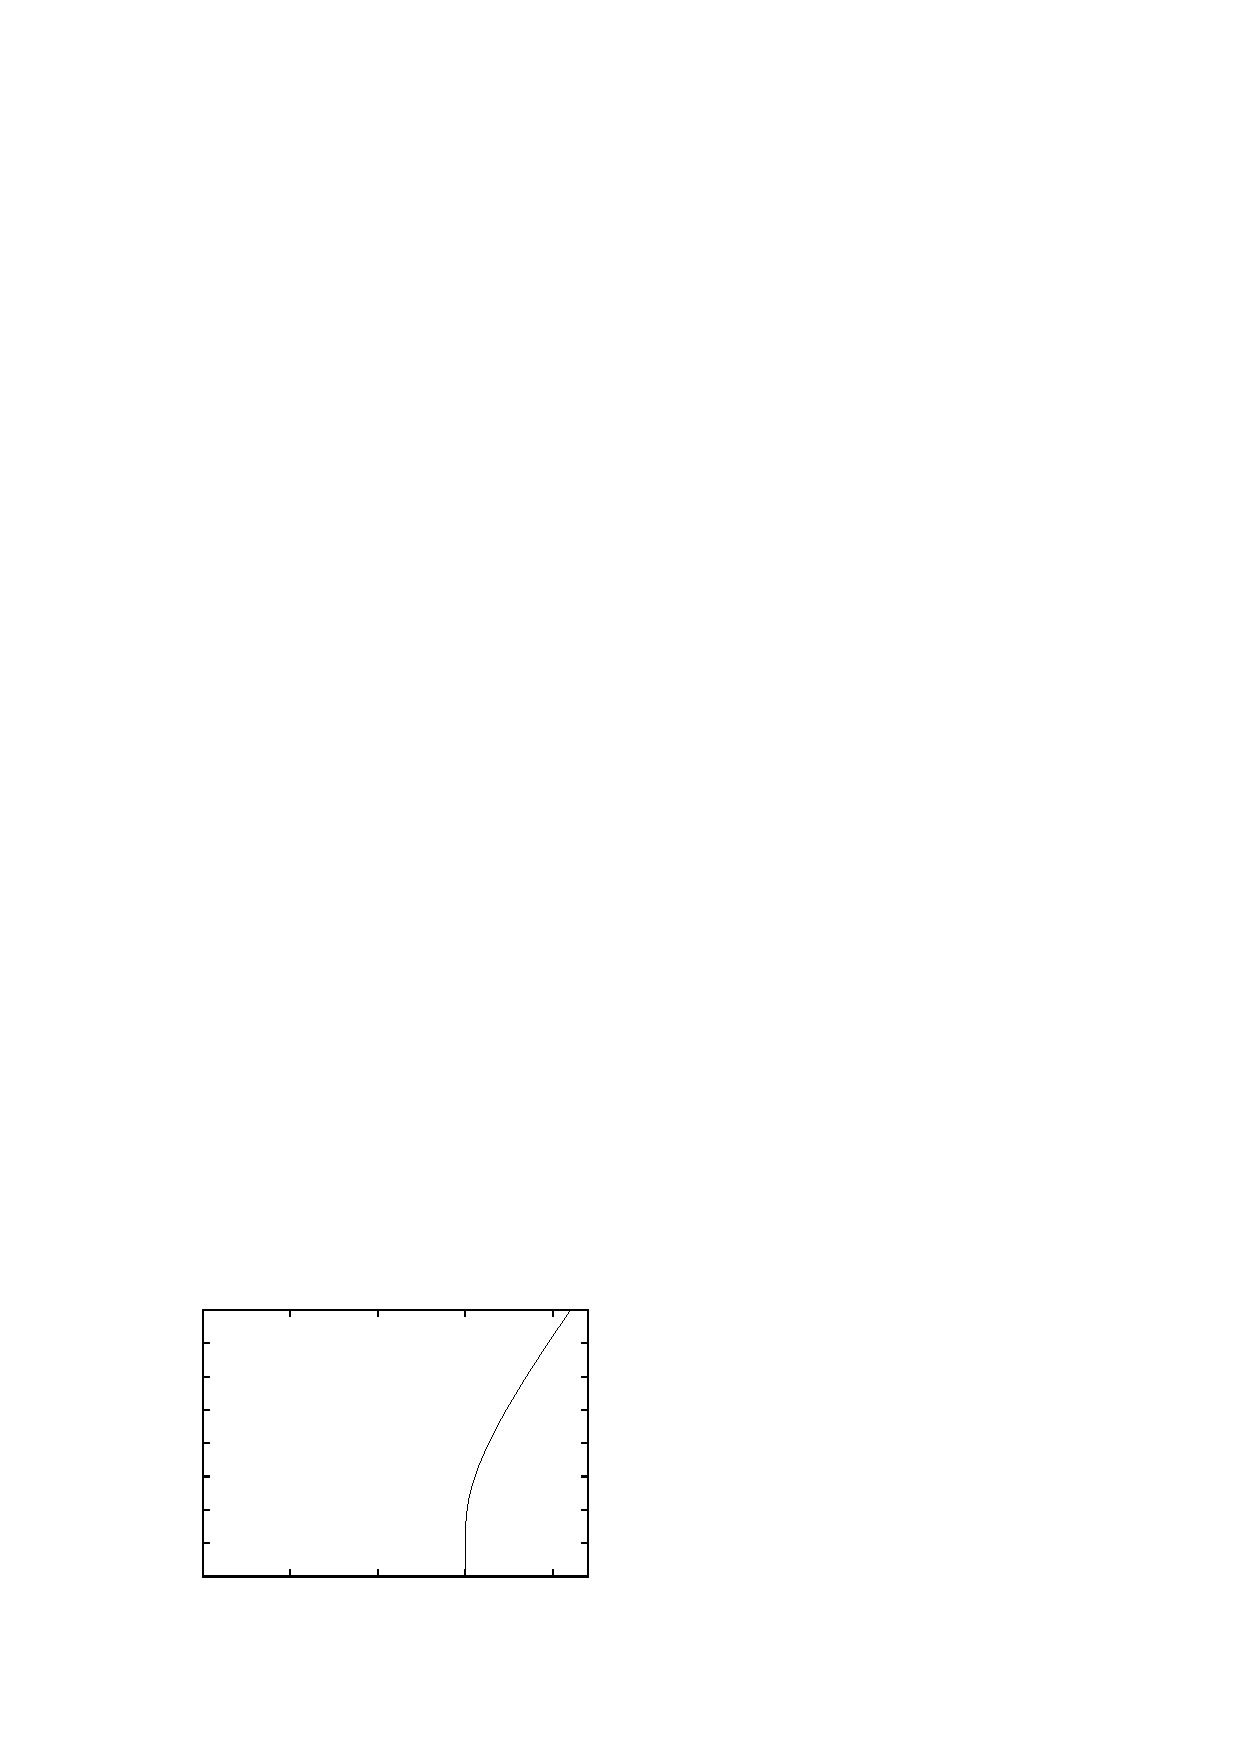
\includegraphics{f_i_curve}}%
    \gplfronttext
  \end{picture}%
\endgroup

\end{center}
  \end{frame}

\begin{frame}{Some observations}
  \begin{itemize}
  \item This tells us that neurons filter their input.
  \item The model doesn't have spike rate adaptation but can be extended.
  \item Other extensions give more realistic behaviour near threshold.
  \item Including the voltage gated channels gives the \cblu{}Hodgkin-Huxley\cbla{} model.
  \end{itemize}
\end{frame}


\begin{frame}{Some observations}
  \begin{itemize}
  \item To make networks we also need a synapse model.
  \item Lots of synapse models use a similar equation.
  \item The equation for the voltage gated channels also use the same equation.
  \end{itemize}
\end{frame}


\begin{frame}{Numerical calculations}

We saw how to integrate the equation numerically. This can be done
using \texttt{MATLAB}, or better, \texttt{Python} or \texttt{Julia}. There are also specialized
packages like \texttt{Brian} in \texttt{Python} or \texttt{GENESIS} / \texttt{NEURON} / \texttt{NEST}.
  
\end{frame}



\begin{frame}{Summary}
  \begin{itemize}
  \item Studied the dynamics of neurons away from threshold.
  \item Discussed chemical gradients.
  \item Looked at the integrate and fire model.
  \item Considered the f-I curve in the integrate and fire model.
  \end{itemize}
\end{frame}



\end{document}

